\documentclass[a4paper,12pt]{article}


\usepackage{amsmath}
\usepackage{graphicx}
\usepackage[capposition=bottom]{floatrow}
\usepackage{amssymb}
\usepackage{caption}

\begin{document}
\title{Triated Methane as an Internal Calibration Source in Xenon Detectors}
\author{Richard Knoche}
\maketitle

\tableofcontents

\section{Introduction to Dark Matter}
Astronomical observations have shown that the rotational velocity of a galaxy remains uniform throughout its entire span.  At the same time astronomers have seen that the luminosity of a galaxy decreases radially outward, suggesting that the mass within a galaxy is concentrated at its center.  This result is quite unexpected.  Our current understanding of gravity predicts rotational speeds to diminish as the distance from the mass increases. So how then do we explain this discrepancy?  One proposed solution is the existence of non-luminous dark matter spread throughout each galaxy. [1] If such a dark matter halo did exist it would account for the higher than predicted rotational velocities in the less luminous regions of galaxies. 

Further evidence of the existence of dark matter can be found in gravitational lensing observations.  Gravitational lensing occurs when light from a very distant source is bent around a massive object, located between the source and the observer, due to relativistic effects. (Figure 1)  By analyzing the distortion of this light the mass of the lens can be determined.  In the cases in which this has been done the luminous matter alone can not account for the amount of distortion seen. [2]

\begin{center}
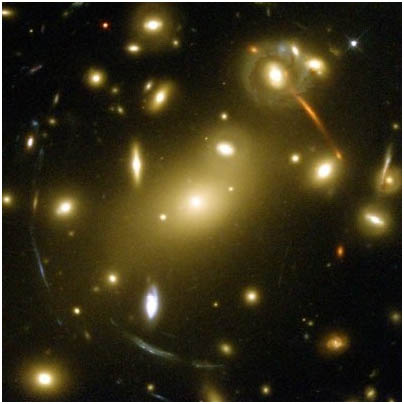
\includegraphics[scale=0.5]{lensing.jpg}
\captionof{figure}{Gravitational Lensing of distant galaxies caused by Abell 2218. Image credit: NASA/JPL}
\end{center}

The observational evidence for the existence of dark matter peaked the curiosity of scientists.  If dark matter does exist, what does it consist of? A fortuitous result known as the WIMP miracle offers one explanation.  During the early stages of the universe dark matter particles must have been created in the primordial soup.  Once the temperature of the universe cooled below the dark matter mass scale the creation of dark matter particles would have ceased.  At this time the dark matter particles which still existed would have continued annihilating with one another.  Thus, as the universe continued to expand, the density of dark matter in the universe began to fall.  As a result, dark matter annihilation became less and less likely.  In this way the final number of dark matter particles became fixed.  This number is directly dependent on the cross section of dark matter annihilation.  Current dark matter density observations predict an annihilation cross section of $ 10^{-9} GeV^{-2} $ -- the same order of magnitude expected for particles interacting only via the weak force. [3] This amazing result is the motivation behind experiments which hope to directly detect the weakly interacting massive particles (or WIMPS) which we call dark matter. 

\section{Liquid Xenon WIMP Detectors}

By definition WIMPs have some probability of scattering off of atomic nuclei through weak interactions.  A detector sensitive enough to such interactions would be able to directly detect these WIMPs.  To pull this off the detector would need to have very low background rates and a large target mass to compensate for the low probability of WIMP scattering.  This makes liquid xenon detectors an ideal candidate for WIMP searches. [4]

The advantages of using xenon in a WIMP detector are numerous.  Xenon has no long lived radioactive isotopes, so it does not contribute to background radiation.  Additionally, xenon's high atomic mass  ($ A \approx 132 $) and dense liquid state (3 $ g/cm^3 $) means that it has a relatively large cross section for detecting WIMPs.

\begin{center}
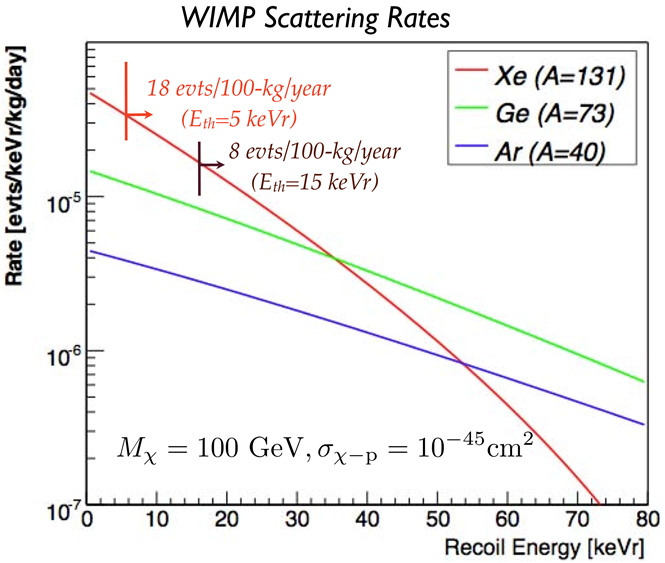
\includegraphics[scale=1]{CrossSections.png}
\captionof{figure}{WIMP scattering rates in different media.  The WIMP-nucleus cross section is proportional to the atomic mass squared, so xenon has a higher cross section than germanium, and germanium has a higher cross section that argon.  Note that the energy spectrum in xenon is softer, so a lower energy threshold is needed.}
\end{center}

In two phase (liquid and gas) xenon detectors there are two distinct types of events -- electron recoils and nuclear recoils.  In electron recoils gamma rays or beta particles recoil off of the electrons in the xenon atoms, producing scintillation light (referred to as S1) and charged particles.  Photo-multiplier tubes can be used to measure the scintillation light, while the charged particles can be drifted to an anode located in the gas phase of the detector.  Once the charged particles are accelerating toward the anode in the xenon gas they will create an electron cascade, producing a second source of scintillation light (referred to as S2).  In a similar fashion, nuclear recoil events will also produce S1 and S2 scintillation.  The key to distinguishing these two types of events lies in the ratio of energy in the S1 and S2 scintillation from each event.  Nuclear recoil events have higher ionization density, leading to a higher recombination probability, resulting in a higher S1 yield. To utilize this distinction it is necessary to calibrate the detector in the fiducial region with the goal of knowing to a certain confidence level which signals are caused by electron recoil events, and what percentage of nuclear recoil events must be thrown out because of overlap of the two spectra.  Data for calibrating LUX's predecessor in this manner is shown in figure three.

\begin{center}
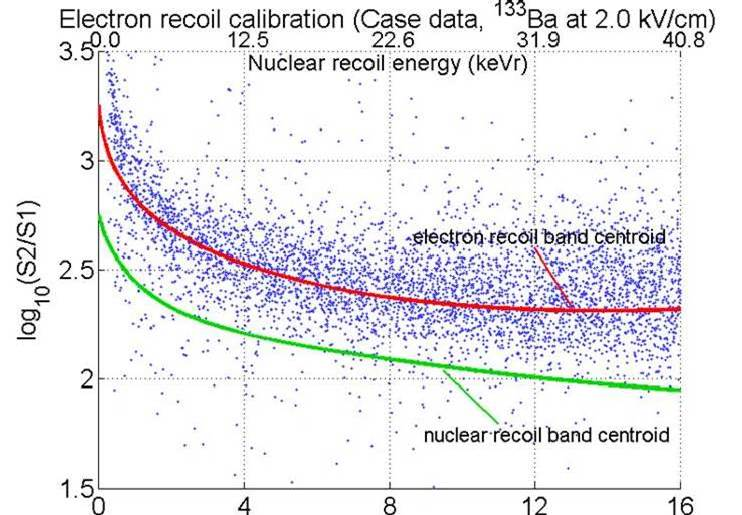
\includegraphics[scale=0.75]{Recoils.jpg}
\captionof{figure}{A plot of electron recoil events generated by an external calibration source in LUX's predecessor LUX-0.1.  This data is used to determine the electron recoil band shown in red, while data from a neutron source (not shown) is used to determine the nuclear recoil band shown in green }
\end{center}


\section{The Large Underground Xenon Detector}

The Large Underground Xenon Detector (LUX) is one experiment utilizing a xenon WIMP detector. [5,6] It is a dual phase time projection chamber containing 350 kg of xenon used as the target mass.  The xenon is cooled by a thermosyphon system until it condenses in the detector.  Inside of the xenon space there is one photo-multiplier tube array submerged in the liquid xenon, another photo-multiplier tube array suspended in the xenon gas, and five wire grids producing an electric field to drift charged particles through the detector.  The location of the S2 signal provides the x and y coordinates of the recoil event, while the time between the S1 and S2 signal provides the z coordinate of the recoil event.  This allows the primary event to be localized within one centimeter in all three spacial dimensions.  The xenon space is shielded by a 300 ton water tank which houses additional photo-multiplier tubes for cosmic ray vetoing. 

\begin{center}
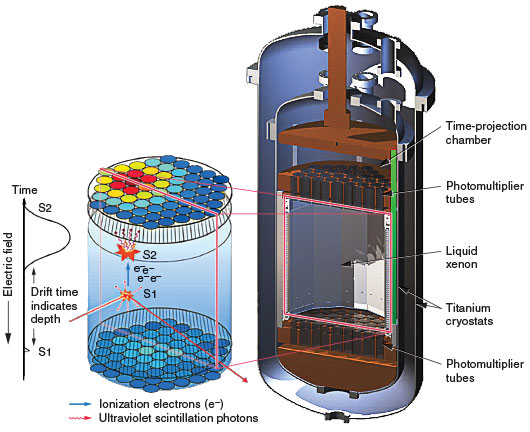
\includegraphics[scale=0.5]{lux.jpg}
\captionof{figure}{Image depicting the internals of the LUX detector.}
\end{center}

\section{Calibration of the Detector}

In order to distinguish dark matter signals in the detector from background signals the detector's response to nuclear recoil events and electron recoil events must be well understood.  It is common to use an external beta emitter such as cesium-137 to achieve this goal.  However, the xenon in LUX has a strong self-shield characteristic (radiation length $ \approx 2.77 $ cm).  While this is convenient for eliminating background radiation, it makes calibrating the inner most regions of the detector a challenge.

To overcome this problem LUX is making use of internal calibration sources.  An ideal internal calibration source would need to be a single beta emitter in the energy range of interest ($ <15 $ keV) which can be dissolved into the liquid xenon in the detector.  Furthermore, the source must be made of a material with low electronegativity so that it will not poison the detector's charge drift length.  Similarly the source can not attenuate the UV scintillation light produced by recoil events in the detector.  To achieve a reliable calibration in all regions of the detector the source would need to have a long enough life time to diffuse throughout the entire detector (a few hours).  Finally, there must be a method for removing the source once the calibration has finished.  This could simply mean waiting for the source to decay if its half life is short, or actively purifying the source out of the detector if its half life is long. [7]

\section{Tritium as an Internal Calibration Source}

Tritium meets several of these requirements.  It is a beta emitter with a Q-value of 18 keV that produces a broad spectrum over the entire energy range of interest.  Its 12.3 year half life means that the source will have plenty of time to dissolve uniformly throughout the detector.  However, this long half life serves as a double edged sword.  Since its half life is on the order of a decade one could not simply wait for it to decay away -- it must be actively removed from the detector when the calibration is completed.  To complicate this matter bare tritium sticks to most surfaces, including materials like teflon, polyethylene, and steel which make up the majority of most xenon detectors.

To make removing the tritium from the detector more feasible we have made use of tritiated methane ($ CH_3T $).  Methane is highly inert due to its fully saturated carbon-hydrogen bonds.  It has a diffusion constant in polyethylene that is 10 times smaller than hydrogen, and it does not capture electrons that will be drifting through the detector.  By replacing one of the hydrogen atoms in a methane molecule with tritium we combine the strength of both of these materials, resulting in the ideal internal calibration source.


\section{Gas Experiments}

To determine the viability of using tritiated methane as an internal calibration source we built a system to inject tritiated methane into a gaseous xenon environment.  This system consists of three sections.  The first section, the xenon space, contains a xenon purifier which uses hot zirconium to remove the tritiated methane, two xenon storage bottles used to move xenon through the system via cryopumping, and a proportional tube used to detect activity within the xenon space.  The second section is a small transfer system which is used to inject consistent amounts of methane into the xenon space with each injection.  The final section consists of a tritiated methane storage bottle used as the source of injections and a SAES MC1-905F methane purifier to remove unwanted contaminates prior to entering the xenon space.

\begin{center}
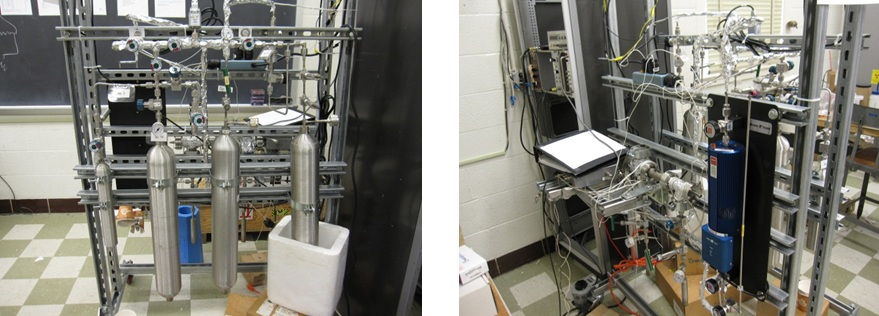
\includegraphics[scale=0.5]{gassys.jpg}
\captionof{figure}{Front and back of the tritiated methane injection system for the gas phase experiments at UMD.}
\end{center}

The primary goal of this experiment was to determine how to maximize our purification efficiency.  There are two factors which dominate this process -- flow rate through the purifier and rest time between subsequent purifications.  High flow rates through the purifier can cool the zirconium inside, while inadequate rest time between purifications can lead to build up of methane on the surface of the zirconium beads.  Both of these situations lead to a decrease in purifier efficiency. 

The first black data point in figure six is our worst purification efficiency, (96\% +/- 1\%) corresponding to our highest flow rate. (8 SLPM compared to the typical ~0.3 SLPM)  While we were unable to control the flow through our experiment as much as we desired, we are at least able to conclude that exceeding the maximum flow rate suggested for the purifier does significantly decrease purification efficiency.

\begin{center}
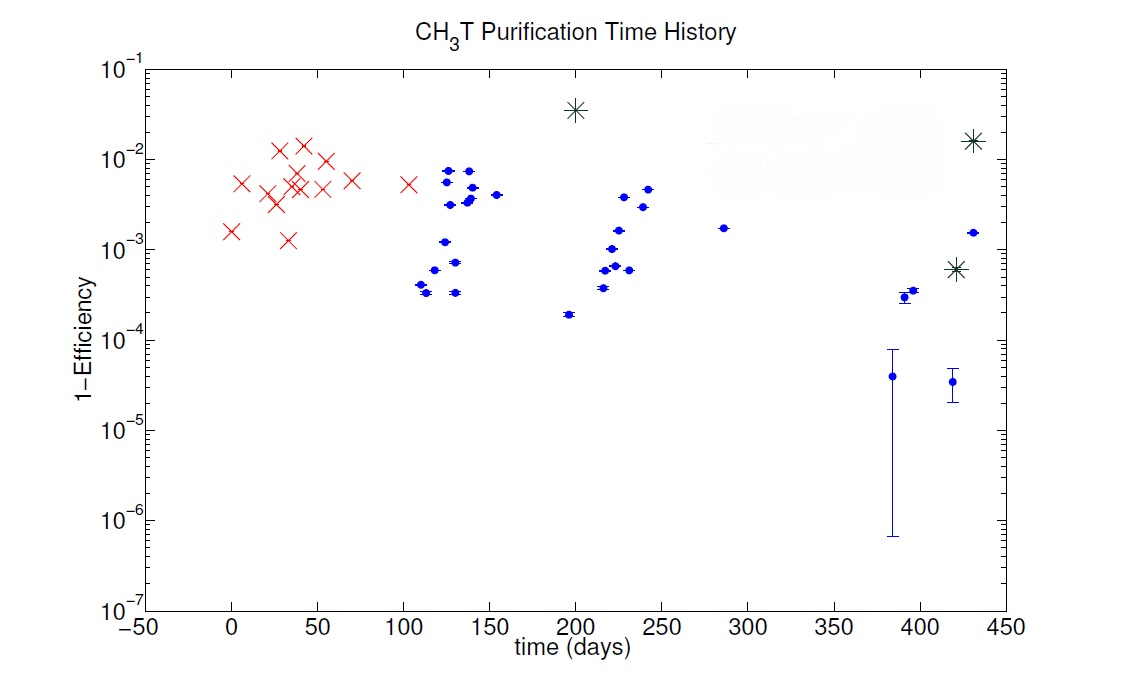
\includegraphics[scale=0.5]{Figone.jpg}
\captionof{figure}{Single pass efficiency of the purifier when removing tritiated methane.  The red and blue points indicate data taken by different students, while the black points indicate data for which the procedures were intentionally altered. }
\end{center}

We found that allowing for ample rest time between purifications does significantly increase purification efficiency. Our best purifications were the first data points in each cluster in figure seven.  We were able to obtain efficiencies of 99.99\% when the purifier was resting for three weeks or longer, and obtained efficiencies of 99\% to 99.9\% when the purifier was used on a daily basis.

\begin{center}
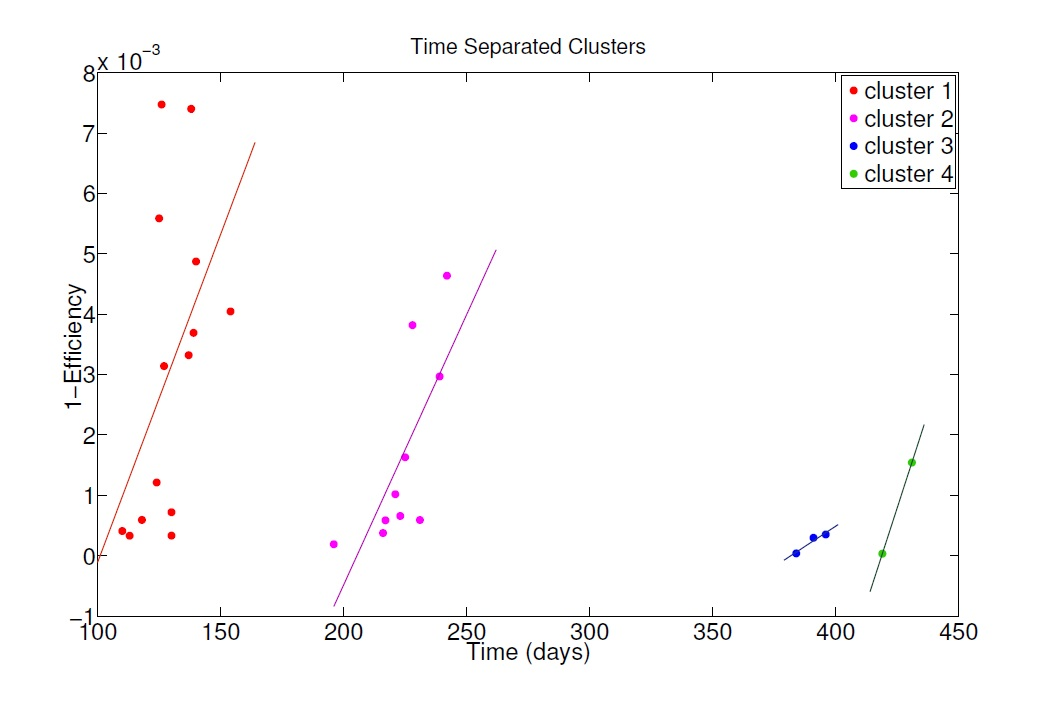
\includegraphics[scale=0.5]{Figfour.jpg}
\captionof{figure}{Time-separated clusters of purifications have an upward trend in purification inefficiency.  Each cluster shown is separated in time by at least three weeks.}
\end{center}

\section{Liquid Experiments}

With the compeletion of the gaseous xenon experiments, we moved on to test removing triated methane from a liquid xenon environment.  To do this we have made use of our liquid xenon system at the University of Maryland.  The system consists of two main sections, the tritiated methane injection system and the liquid xenon system.  We will first discuss the set up of the tritium injection system, pictured below.

\begin{center}
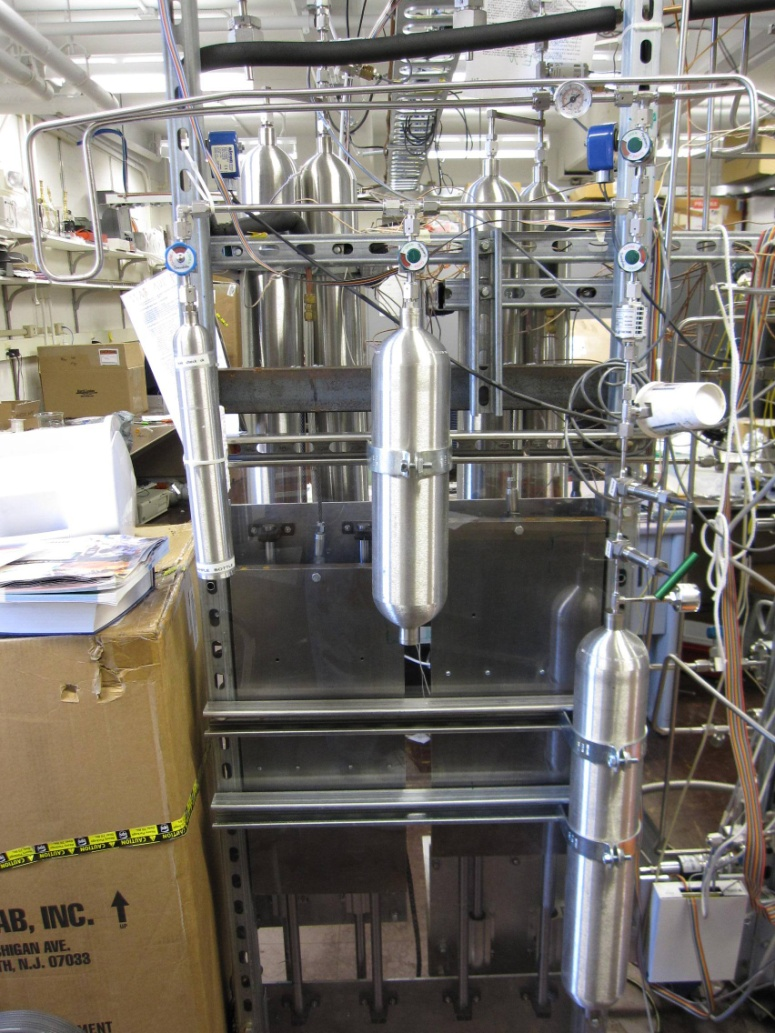
\includegraphics{UMDIS.png}
\captionof{figure}{The tritium injection system for the liquid phase experiments at UMD.}
\end{center}

The injection system begins at the tritiated methane storage bottle.  This bottle is double valved for safety reasons.  As with the gaseous experiments, we have a SAES MC1-905F methane purifier in series with the storage bottle.  Following the methane purifier there is a series of injection volumes branching off to the left.  These injection volumes are designed to inject the desired amount of tritiated methane into the xenon system.  The last component of the injection system is located above the injection volumes.  This plumbing is used to collect all of the tritiated methane from the injection volume via cyropumping.  After the plumbing has warmed, the xenon circulating outside of the injection system is rerouted through the cryopump plumbing to sweep all of the tritiated methane into the xenon system.

The second section of our system, the liquid xenon system, is pictured below.

\begin{center}
\includegraphics[scale=0.5]{cryo.png}
\captionof{figure}{The liquid xenon system at UMD.}
\end{center}

In the liquid xenon system, a refrigerator cold head cools the plumbing in which the xenon circulates.  The cooled xenon then condenses and drips into a liquid xenon storage vessel.  Inside of the liquid xenon storage vessel are two PMTs that are looking at each other.  Once the vessel is filled both of these PMTs are submerged in the liquid xenon.  Note that this means the system at UMD is a single phase detector, rather than a dual phase detector like LUX.  It should be noted that in the plumbing leading to the liquid xenon system there is a SAES Zirconium getter (pcf4c3r1) used to purify the tritiated methane out of the system when desired.

\subsection{Liquid Experiments Results}

Using the lessons learned from the gaseous xenon experiments we were able to remove over 99.9\% of any tritiated methane that was injected into our liquid xenon system.  To illustrate this point, the spectra seen by our PMTs before an injection, after an injection, and after purification are shown in figure ten.

\begin{center}
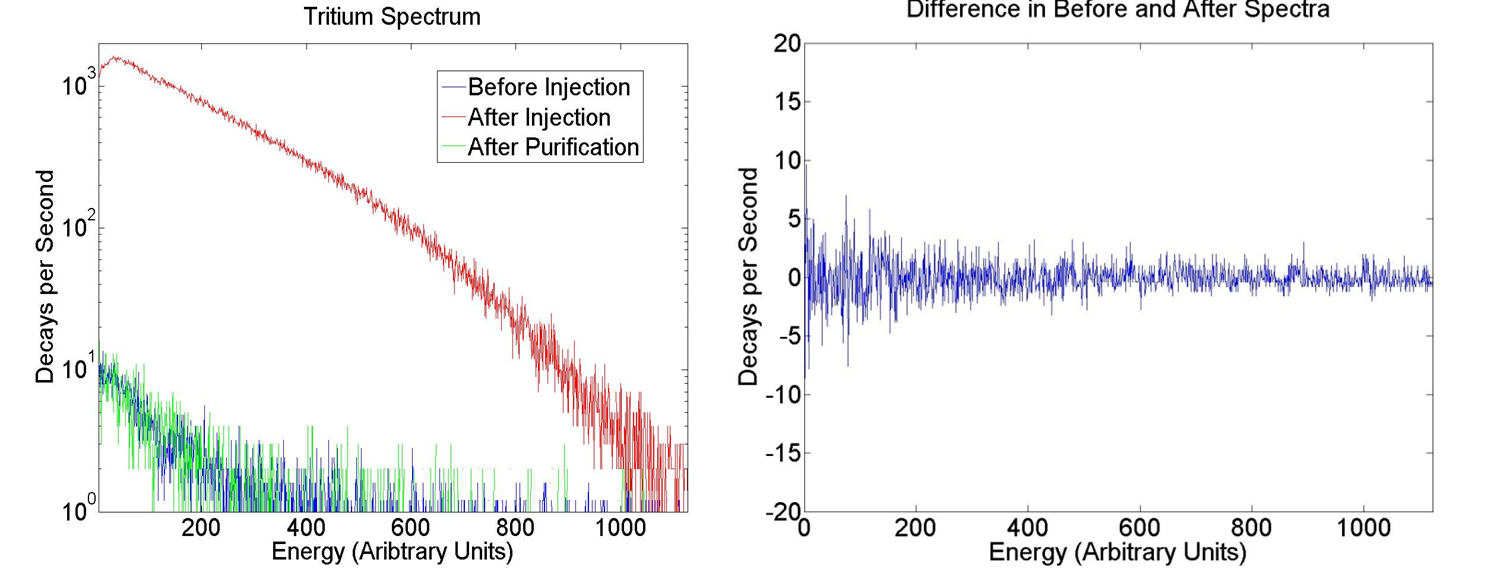
\includegraphics[scale=0.5]{spectra.png}
\captionof{figure}{Left: Overlay of spectra seen by PMTs in the liquid xenon detector.  The blue spectrum is what is seen by the PMTs prior to injecting tritium, the red spectrum is what is seen by the PMTs after injecting tritium, and the green spectrum is what is seen by the PMTs after purifying the xenon to remove any injected tritiated methane.  Right: The difference between the before injection and after purification spectra. }
\end{center}


We were able to repeat the injection and purification procedures many times without seeing any rise in the residual background of our system.  Figure eleven illustrates this point.  So far we have injected over ten thousand becquerel of activity without seeing any rise in residual background rates.

\begin{center}
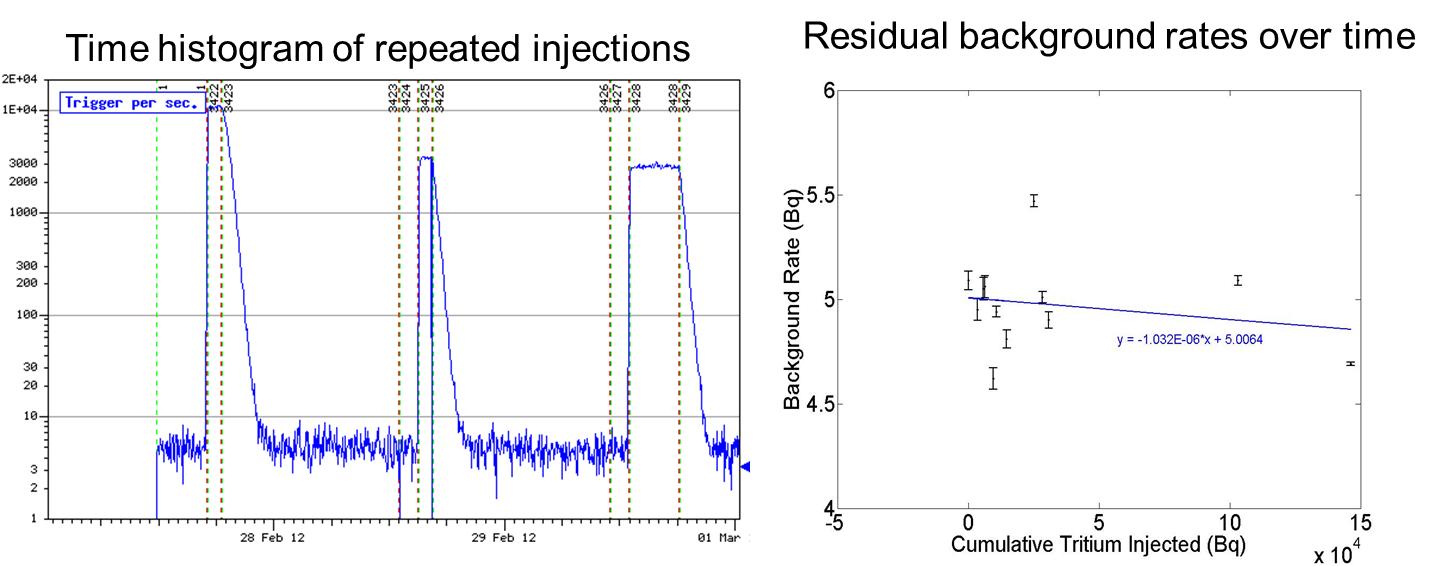
\includegraphics[scale=0.5]{backgrounds.png}
\captionof{figure}{Left: Time histogram of three of our tritiated methane injections. The y-axis of this figure is count rate, while the x-axis is time.  Right:  Residual background rates over time in our detector after purifying the tritiated methane out of the xenon.  }
\end{center}

\section{Diffusion Experiments}

Will write up at end of current experiments

\section{Tritium Injection System for LUX}

With the knowledge we obtained from our experiments at UMD we have designed and built a tritium injection system for the purpose of calibrating the LUX detector.  This tritium injection system consists of a tritiated methane bottle, a methane purifier, and subsequent expansion volumes to fine tune the amount of activity being injected.  The tritiated methane bottle contains a mixture of tritiated methane and dekryptonated xenon gas.  The dekyrpotonated gas is included in the bottle to raise its pressure and ensure no backward flow from the LUX system into the bottle.

PICTURE OF INJECTION SYSTEM, AND MAYBE PLUMBING DIAGRAM (Dont have this picture yet)

To use the system an operator must first determine which expansion volumes are required to obtain the desired injection activity.  Once these injection volumes have been filled with tritiated methane, the tritiated methane bottle is isolated and the LUX xenon gas flow is diverted through the expansion volumes.  This sweeps the tritiated methane out of the injection system and into the LUX detector.  Since LUX's standard operating mode has a xenon purifier included in its flow path this tritiated methane will be removed from the system as it circulates. 

\begin{thebibliography}{1}

\bibitem{D'Amico} \emph{Dark Matter Astrophysics}. D'Amico, Guido et al. arXiv:0907.1912[astro-ph.CP] 
\bibitem{Wu} \emph{A Comparison of Different Cluster Mass Estimates: Consistency or Discrepancy?}. Wu et al.  Monthly Notices of the Royal Astronomical Society 301 (3):861-971.  arXiv:astro-ph/9808179
\bibitem{Griest} \emph{Supersymmetric Dark Matter}.  Griest et al.  Phys. Rept. 333 (2000) 167-182
\bibitem{Aprile} \emph{Liquid Xenon Detectors for Particle Physics and Astrophysics}.  E. Aprile, T.Doke. Rev. Mod. Phys. 82 (2010) 2053-2097
\bibitem{McKinsey} \emph{The LUX Dark Matter Search}.  McKinsey et al.  Journal of Physics: Conference Series 203 (2010) 012026
\bibitem{Fiorucci} \emph{Status of the LUX Dark Matter Search}. Fiorucci et al.  AIP Conference Proceedings 1200 (2010) 977
\bibitem{Kastens} \emph{Calibration of a Liquid Xenon Detector with Kr-83} Kastens et al. Phys. Rev. C 80 (2009) 045809


\end{thebibliography}


\end{document}

